\documentclass[11pt,a4paper]{report}
\usepackage[latin1]{inputenc}
\usepackage{amsmath}
\usepackage{amsfonts}
\usepackage{mathtools}
\usepackage{array}
\usepackage{pifont}
\usepackage{ifsym}
\usepackage{booktabs}
\usepackage{listings}
\usepackage{amssymb}
\usepackage{graphicx}
\usepackage{longtable}
\usepackage{tabularx}
\usepackage{enumitem}
\usepackage{xcolor}
\usepackage{url}
\usepackage[margin=0.8in]{geometry}
\usepackage[toc,page]{appendix}
\usepackage{etoolbox}
\usepackage{morefloats}
\usepackage{multirow}
\usepackage[hidelinks]{hyperref}
\usepackage{float} % Allows putting an [H] in \begin{figure} to specify the exact location of the figure
\usepackage{verbatim}
\usepackage{listings}

\usepackage{fullpage}

\definecolor{green}{rgb}{0,0.6,0}
\definecolor{mygray}{rgb}{0.5,0.5,0.5}
\definecolor{mymauve}{rgb}{0.58,0,0.82}
\definecolor{orange}{RGB}{255,127,0}
\colorlet{punct}{red!60!black}
\definecolor{background}{HTML}{EEEEEE}
\definecolor{delim}{RGB}{20,105,176}
\definecolor{Blue}{HTML}{1589FF}
\definecolor{OliveGreen}{HTML}{6CC417}
\definecolor{Maroon}{HTML}{810541}
\colorlet{numb}{magenta!60!black}

\lstset{ %
  backgroundcolor=\color{white},   % choose the background color; you must add \usepackage{color} or \usepackage{xcolor}
  breakatwhitespace=false,         % sets if automatic breaks should only happen at whitespace
  breaklines=true,                 % sets automatic line breaking
  captionpos=b,                    % sets the caption-position to bottom
  commentstyle=\color{green},    % comment style
  deletekeywords={...},            % if you want to delete keywords from the given language
  escapeinside={\%*}{*)},          % if you want to add LaTeX within your code
  extendedchars=true,              % lets you use non-ASCII characters; for 8-bits encodings only, does not work with UTF-8
  keepspaces=true,                 % keeps spaces in text, useful for keeping indentation of code (possibly needs columns=flexible)
  keywordstyle=\color{blue},       % keyword style
  language=Octave,                 % the language of the code
  morekeywords={*,...},            % if you want to add more keywords to the set
  rulecolor=\color{black},         % if not set, the frame-color may be changed on line-breaks within not-black text (e.g. comments (green here))
  showspaces=false,                % show spaces everywhere adding particular underscores; it overrides 'showstringspaces'
  showstringspaces=false,          % underline spaces within strings only
  showtabs=false,                  % show tabs within strings adding particular underscores
  stepnumber=2,                    % the step between two line-numbers. If it's 1, each line will be numbered
  stringstyle=\color{mymauve},     % string literal style
  tabsize=2,                       % sets default tabsize to 2 spaces
  title=\lstname                   % show the filename of files included with \lstinputlisting; also try caption instead of title
}

\lstset{language=PHP,
    basicstyle=\ttfamily,
    keywordstyle=\bfseries\color{blue},
    showstringspaces=false,
    morekeywords={}
} 

\renewcommand{\ttdefault}{pcr}


\DeclareUrlCommand{\bfurl}{\def\UrlFont{\bfseries\ttfamily}}

\usepackage{lipsum} % Used for inserting dummy 'Lorem ipsum' text into the template
\usepackage{etoolbox}
\apptocmd{\sloppy}{\hbadness 10000\relax}{}{}

\linespread{1.2} % Line spacing

\graphicspath{{img/}} % Specifies the directory where pictures are stored

\lstset{ %
	basicstyle=\normalfont\ttfamily,
    numbers=left,
    numberstyle=\scriptsize,
    stepnumber=1,
    numbersep=8pt,
    showstringspaces=false,
    breaklines=true,
    frame=single,
    xleftmargin=1em,
    framexleftmargin=1.5em,
    backgroundcolor=\color{background}
}

\lstdefinelanguage{json}{
    literate=
     *{0}{{{\color{numb}0}}}{1}
      {1}{{{\color{numb}1}}}{1}
      {2}{{{\color{numb}2}}}{1}
      {3}{{{\color{numb}3}}}{1}
      {4}{{{\color{numb}4}}}{1}
      {5}{{{\color{numb}5}}}{1}
      {6}{{{\color{numb}6}}}{1}
      {7}{{{\color{numb}7}}}{1}
      {8}{{{\color{numb}8}}}{1}
      {9}{{{\color{numb}9}}}{1}
      {:}{{{\color{punct}{:}}}}{1}
      {,}{{{\color{punct}{,}}}}{1}
      {\{}{{{\color{delim}{\{}}}}{1}
      {\}}{{{\color{delim}{\}}}}}{1}
      {[}{{{\color{delim}{[}}}}{1}
      {]}{{{\color{delim}{]}}}}{1},
}

\begin{document}

\begin{titlepage}

\begin{center}

\includegraphics[width=0.5\textwidth]{img/University_Logo}\\

\textsc{\LARGE Swansea University }\\[0.5cm]
\textsc{\large MEng Computing }\\[2cm]

{ \huge \bfseries Group Project CS-M04}\\[0.2cm]
\textsc{\large Team Structure, Methodology, Requirements and Specifications}\\[1.5cm]

\begin{minipage}{0.4\textwidth}
\begin{flushleft}

\emph{Authors:}\\
Adam \textsc{Barrell} {\scriptsize \emph{(632975)}} \\
Thomas \textsc{Milner} {\scriptsize \emph{(637755)}} \\
Lewis \textsc{Hancock} {\scriptsize \emph{(xxxxxx)}} \\
Christopher \textsc{Lewis} {\scriptsize \emph{(xxxxxx)}} \\

\end{flushleft}
\end{minipage}
\begin{minipage}{0.4\textwidth}
\begin{flushright}

\emph{Supervisor:}\\
Parisa \textsc{Eslambolchilar}

\end{flushright}
\end{minipage}\\[1.3cm]

{\today}
\end{center}

\end{titlepage}

\newpage
\setcounter{page}{1}
\pagenumbering{roman}
\tableofcontents

\newpage
\setcounter{page}{1}
\pagenumbering{arabic}
\chapter*{Introduction}
\addcontentsline{toc}{chapter}{Introduction}

\label{sec:introduction}
\section{Term Definitions}
\label{sec:term-definitions}
\section{Project Overview}
\label{sec:project-overview}

\chapter{Design}
\label{sec:design}

\section{Web Portal}
\label{sec:web-portal-design}
% User Interface Design
% UML Diagrams
% Descriptions of each module
% Technology Choices

\subsection{Rejected Designs}
\label{sec:rejected-designs}

\subsection{Chosen Design}
\label{sec:chosen-designs}


\section{Android Application}
\label{sec:android-design}
% User Interface Design
% UML Diagrams
% Descriptions of each class
% Technology Choices

\subsection{Rejected Designs}
\label{sec:rejected-designs}

\subsection{Chosen Design}
\label{sec:chosen-designs}


\section{API}
\label{sec:api-design}

The API is the crucial link between the Website, Application and Database. It was important that the correct design and technology was selected to make that link as seamless as possible. 

\subsection{Possible Designs}
\label{sec:api:rejected-designs} %Phalcon Framework. SOAP API's.
When work started on the API the first descision that needed to be made was on the protocal for the API. There are several popular API protocals including;

\begin{itemize}
\item SOAP
\item REST
\item JSON-RPC 
\item XML-RPC \ldots
\end{itemize}

The most popular two are SOAP and REST. SOAP was originally defined as `Simple Object Access Protocol' and is the sucssesor to XML-RPC (XML Remote Procedure Call). It uses a XML document for its message which is sent over either the HTTP or SMTP application protocals. The XML document which is transmitted with a SOAP request has several parts. The document will start with an `Envelope' which contains all of the data. Inside the `Envelope' there is an optional `Header', a compolsary `Body' which contains request data, and an optional `Fault' which contains any errors which have occured. Listing \ref{lst:soap} shows an example of a SOAP request.

\lstset{language=xml,
keywordstyle=\color{Maroon},
commentstyle=\color{OliveGreen},
showstringspaces=false, tabsize=4, breaklines=true, showspaces=false, stringstyle=\color{Blue}}

\begin{lstlisting}[captionpos=b, caption=An example SOAP request., label=lst:soap, frame=single]
POST /InStock HTTP/1.1
Host: www.example.org
Content-Type: application/soap+xml; charset=utf-8
Content-Length: 299
SOAPAction: "http://www.w3.org/203/05/soap-envelope"
 
<?xml version="1.0"?>
<soap:Envelope xmlns:soap="http://www.w3.org/203/05/soap-envelope">
  <soap:Header>
  </soap:Header>
  <soap:Body>
    <m:GetStockPrice xmlns:m="http://www.example.org/stock">
      <m:StockName>IBM</m:StockName>
    </m:GetStockPrice>
  </soap:Body>
</soap:Envelope>
\end{lstlisting}

REST, on the other hand, is a stateless system which comunicates via URI's, any media (such as JSON or XML) and HTTP Methods. REST stands for Representational State Transfer, which implys a representation of the current state must be transfered to the API with reach request. A REST request to retrive an object can be as simple as \lstinline$GET http:\\example.com\api\users$. The simplicity of REST lends its self to many situations and makes it easy to adapt to specific cases. 

\subsection{Chosen Desgin}
For the API it was decided to harness the REST protocal. The decision was made after analysing both SOAP and REST and the advantages and disadvantages of both. In the end the overly veribose nature of SOAP led to the decision of a REST api.  The ability to use JSON with REST requests was also a deciding factor as this gretly reduced the workload when comunicating with the API from JavaScript. 

\subsection{UML Diagrams}
\label{sec:api:uml}

\subsection{Classes}
\label{sec:api:class}
The API has several `Model' classes to represent the Database tables and the objects that are stored within them. The objects are related through the database and can retrieve the related models through method calls. The relations between the models is shown in Figure \ref{fig:datamodels}, where every model is a possible entry point. Using these models it is possible to, for example, use an `English Walk Description' to return all related 'Waypoint Images'. 

\begin{figure}[H]
    \centering
    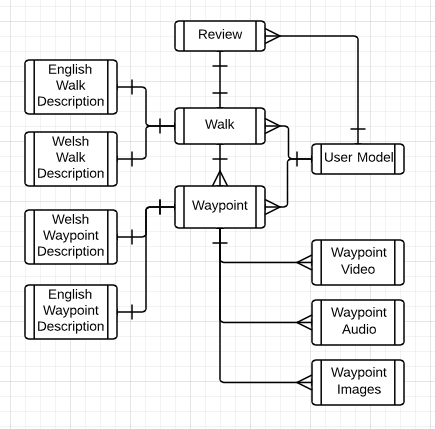
\includegraphics[width=0.5\textwidth]{DataModels}
    \caption{The Data Model and their relations.}
    \label{fig:datamodels}
\end{figure}

The API has several main object collections, which are `Walks', `Waypoints', `Users', `Waypoint Images', `Waypoint Audio', `Waypoint Video', `Walk Reviews' and `Sessions'. Each collection has a specific route in the API which maps to a collection controller. When a route is called a method in the revelvent controller is called. The method is passed a variable called \$app. This contains the requets and response objects. When the controller has completed its work it writes the response to the \$app object and returns to the index file which initally handled the request. If there is no more work to be done the \$app object sends the response. 

\begin{figure}[H]
    \centering
    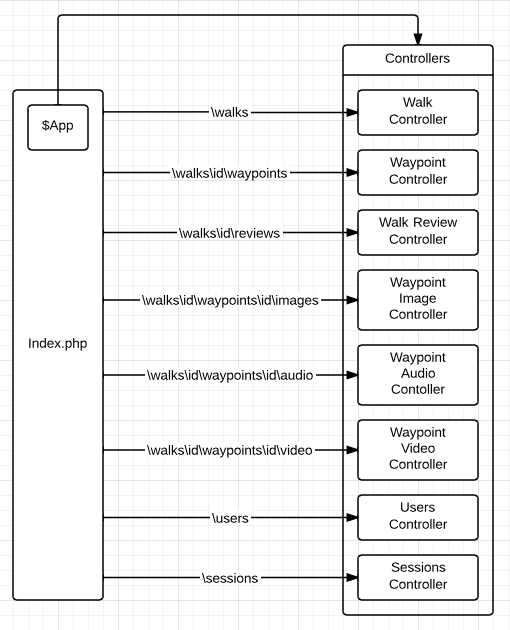
\includegraphics[width=0.5\textwidth]{ControllerRoutes}
    \caption{The connection between routes and controllers.}
    \label{fig:controllerroutes}
\end{figure}

\subsection{Technology Choices}
\label{sec:api:techChoices}

\begin{description}
\item[Paris] - Paris is an ORM (Object Relation Mapper) which provided a layer of abstraction between the database and the API. Rather than writing SQL queries to retrieve an object it makes it possible to use model objects to and methods to retrieve the objects.  
\item[Slim Framework] - The slim framework was chosen as the underlying framework of the API. Slim provides many low-level function which are critical to the production of a reliable API in a small and efficient package. Before it was settled on an alternative framework called Phalcon was trialed, but it proved to be overly complex and overwhelming compared to the relative simplicity of Slim. 
\item[PHP] - This is the language on which Slim runs. It is a popular free and open source web programming langauage. It has great support and is widly used through the world. Alternatives included C\#.NET which is a closed source and closed platform product from Microsoft. Due to the licensing fees and extra costs involved PHP quickly came to light as the best choice. 
\item[Apache] - This is the web server which handles request and responses for the API. It recieves requests and passes them on to the PHP runtime for the API. Apache is the best known and most widely used web server in the world. The alternatives were Nginx and IIS. IIS is limited to Microsfts platforms and Nginx, while well respected, is still an emerging presence in the market. 
\item[Linux] - Linux is the operating system which powers the API server. Linux is free and open source and is the most popular platfrom for operating a server.
\item[JSON] - JavaScript Object Notation (JSON) is a media format which is used to represent JavaScript objects as plain text. It can be used to represent far more than just JavaScript objects however. 
\end{description}

\section{Database}
\label{sec:database-design}
% UML Diagrams
% Descriptions of each entity

\subsection{Rejected Designs}
\label{sec:rejected-designs}

\subsection{Chosen Design}
\label{sec:chosen-designs}

\chapter{Testing}
\label{sec:testing}
\section{Unit Testing}
\label{sec:unit-testint}
\section{Acceptance Testing}
\label{sec:acceptance-testint}

\chapter{User Manual}
\label{sec:user-manual}

\section{API}

\section{Web Portal}

\section{Android Application}

\chapter{Reflective Account}
\label{sec:reflective-account}
\section{Problem Solving}
\label{sec:problem-solving}
\section{Learning Experience}
\label{sec:learning-experience}
\section{Risk Analysis Review}
\label{sec:risk-analysis-review}
\subsection{Anticipated Risks}
\label{sec:anticipated-risks}
\subsection{Un-Anticipated Risks}
\label{sec:unanticipated-risks}
\section{Schedule Review}
\label{sec:schedule-review}
\section{Methodology Review}
\label{sec:methodology-review}
\section{Goals Achieved}
\label{sec:goals-achieved}
\section{Improvements}
\label{sec:improvements}

\chapter*{Summary}
\label{sec:summary}
\addcontentsline{toc}{chapter}{Summary}

%References as subsection
\newpage
\bibliographystyle{plain}
\bibliography{bibliography}

\appendix

\end{document}
